\documentclass[border=10pt]{standalone}

\usepackage{tikz}
\usepackage{tikzsymbols}
\usetikzlibrary{calc,patterns,shapes.geometric}

\def\centerarc[#1](#2)(#3:#4:#5){\draw[#1] ($(#2)+({#5*cos(#3)},{#5*sin(#3)})$) arc (#3:#4:#5);}

\begin{document}
	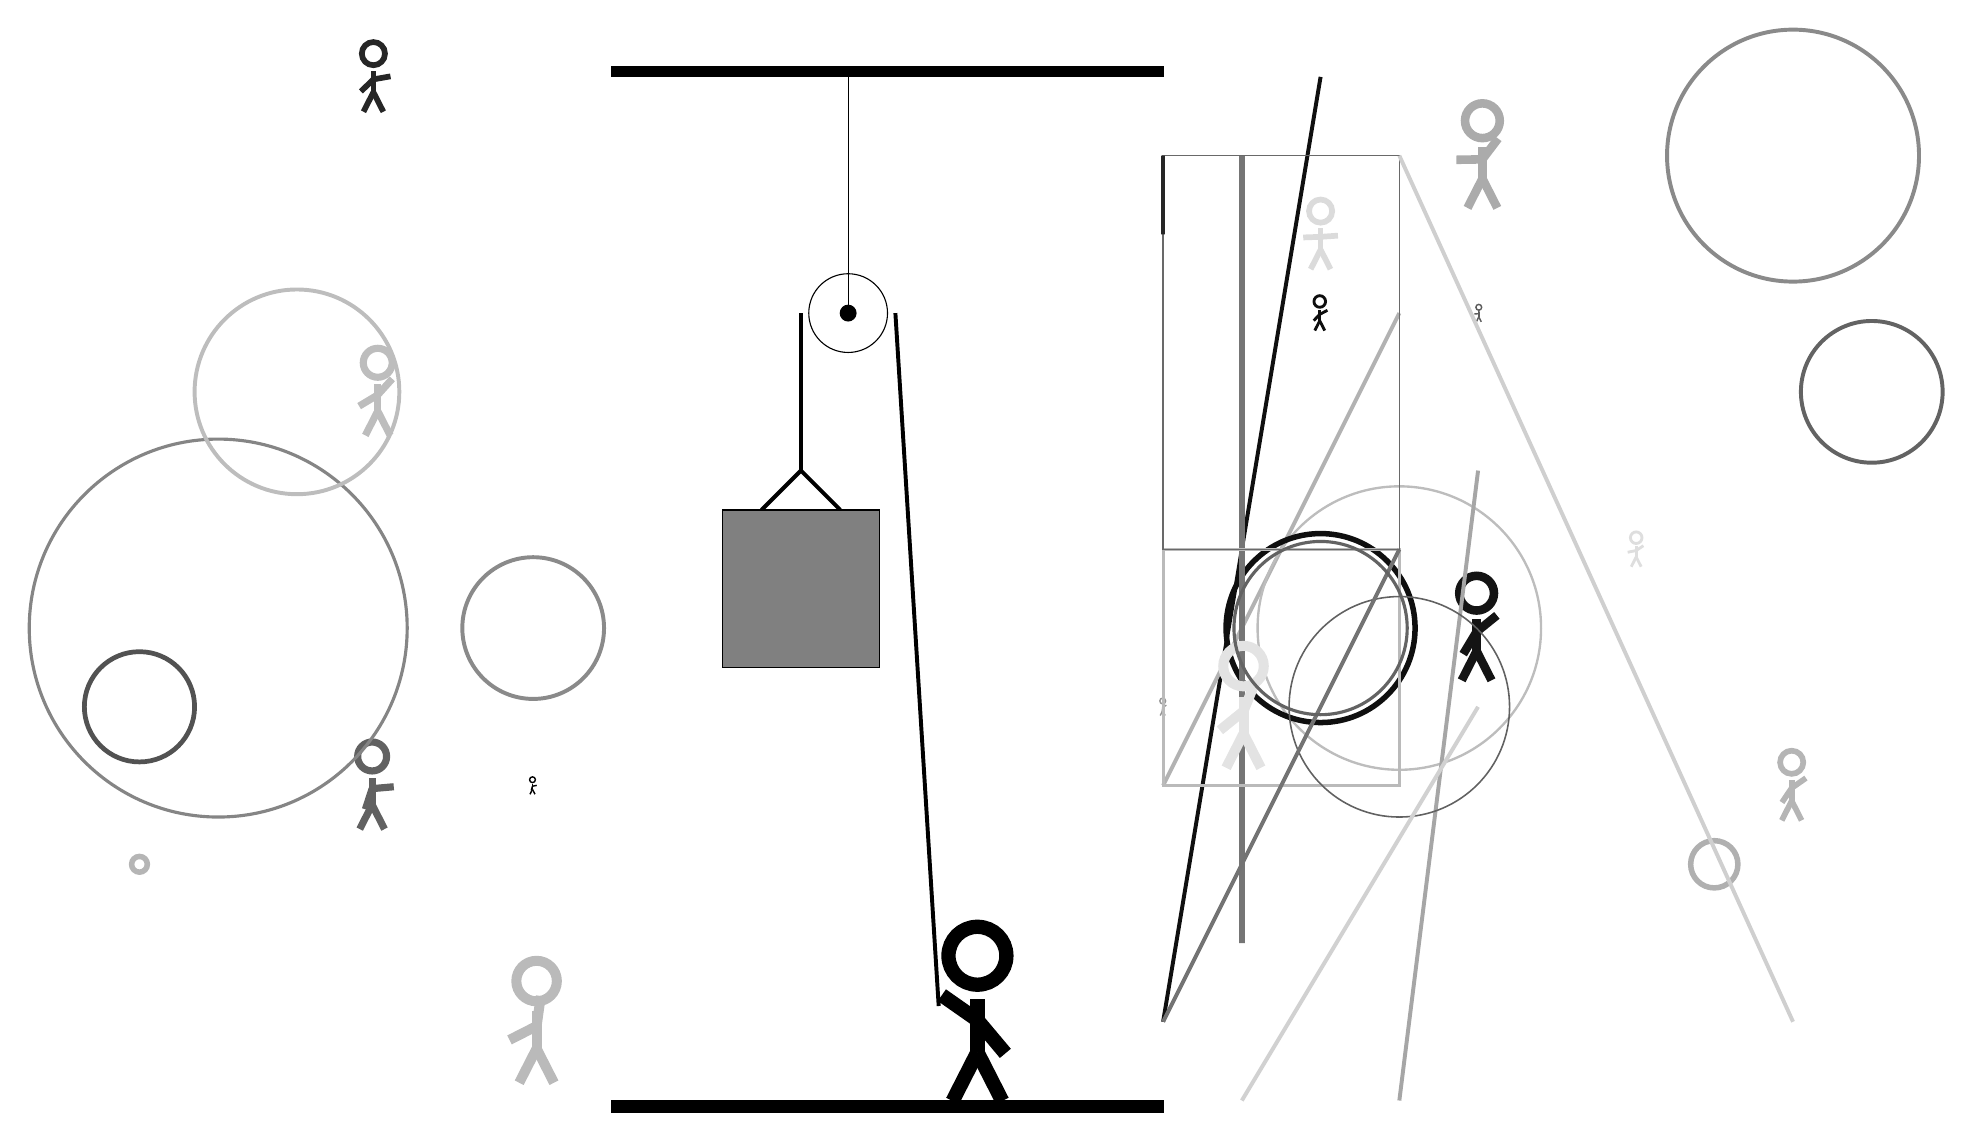
\begin{tikzpicture}
		%%%%% START %%%%%
		
		\draw[fill=black] (-2, 10) rectangle (5, 10.125);
		
		\draw[line width=0.5mm, color=black!94](7, 10) -- (5, -2);
		
		\node[line width=0.2mm, color=black!92] at (9, 3) {\Strichmaxerl[6][59][39]};
		\node[line width=0.7mm, color=black!62] at (-5, 1) {\Strichmaxerl[5][72][5]};
		\draw[line width=0.5mm, color=black!30](5, 1) -- (8, 7);
		\draw [line width=0.6mm, color=black!68](-8, 2) circle (0.7);
		\node[line width=0.5mm, color=black!26] at (-5, 6) {\Strichmaxerl[5][31][48]};
		
		\node[line width=0.7mm, color=black!14] at (7, 8) {\Strichmaxerl[4][2][4]};
		\node[line width=0.4mm, color=black!41] at (5, 2) {\Strichmaxerl[1][83][32]};
		\draw [line width=0.3mm, color=black!26](8, 3) circle (1.8);
		\draw [line width=0.5mm, color=black!46](13, 9) circle (1.6);
		
		\node[line width=0.7mm, color=black!85] at (-5, 10) {\Strichmaxerl[4][44][10]};
		\draw [line width=0.7mm, color=black!94](7, 3) circle (1.2);
		\node[line width=0.7mm, color=black!64] at (9, 7) {\Strichmaxerl[1][2][88]};
		
		\draw[line width=0.7mm, color=black!54] (6, -1) rectangle (6, 9);
		\node[line width=0.5mm, color=black!29] at (13, 1) {\Strichmaxerl[4][56][35]};
		\draw [line width=0.5mm, color=black!46](-3, 3) circle (0.9);
		
		\node[line width=0.3mm, color=black!99] at (-3, 1) {\Strichmaxerl[1][74][10]};
		\draw [line width=0.4mm, color=black!48](-7, 3) circle (2.4);
		\draw[line width=0.4mm, color=black!27] (5, 1) rectangle (8, 4);
		\draw[line width=0.5mm, color=black!35](8, -3) -- (9, 5);
		\draw [line width=0.2mm, color=black!62](8, 2) circle (1.4);
		
		\node[line width=0.4mm, color=black!95] at (7, 7) {\Strichmaxerl[2][46][28]};
		\draw[line width=0.5mm, color=black!18](9, 2) -- (6, -3);
		\node[line width=0.5mm, color=black!11] at (6, 2) {\Strichmaxerl[7][39][68]};
		\draw [line width=0.5mm, color=black!26](-6, 6) circle (1.3);
		\draw [line width=0.7mm, color=black!31](12, 0) circle (0.3);
		\node[line width=0.4mm, color=black!33] at (9, 9) {\Strichmaxerl[6][1][53]};
		\node[line width=0.3mm, color=black!27] at (-3, -2) {\Strichmaxerl[7][27][82]};
		\draw [line width=0.5mm, color=black!61](14, 6) circle (0.9);
		
		\node[line width=0.5mm, color=black!13] at (11, 4) {\Strichmaxerl[2][11][34]};
		\draw [line width=0.7mm, color=black!29](-8, 0) circle (0.1);
		
		\draw[line width=0.5mm, color=black!55](5, -2) -- (8, 4);
		\draw [line width=0.4mm, color=black!61](7, 3) circle (1.1);
		
		\draw[line width=0.2mm, color=black!59] (5, 9) rectangle (8, 4);
		
		\draw[line width=0.5mm, color=black!85] (5, 8) rectangle (5, 9);
		\draw[line width=0.5mm, color=black!19](8, 9) -- (13, -2);
		
		\draw (1, 7) circle (0.5);
		\draw[fill=black] (1, 7) circle (0.1);
		\draw (1, 10) -- (1, 7);
		
		\draw[line width=0.5mm] (-0.1, 4.5) -- (0.4, 5.0) -- (0.9, 4.5);
		\draw[fill=black!50] (-0.6, 4.5) rectangle (1.4, 2.5);
		
		\draw[line width=0.5mm] (0.4, 7) -- (0.4, 5.0);
		\centerarc[line width=0.5mm](1, 7)(0:180:0.6);
		\draw[line width=0.5mm](1.6, 7) -- (2.15, -1.8);
		
		\node at (2.6, -1.9) {\Strichmaxerl[10][-35][-50]};
		
		\draw[fill=black] (-2, -3) rectangle (5, -3.15);
		
		%%%%% END %%%%%
	\end{tikzpicture}
\end{document}